\documentclass[11pt, oneside]{article} 
\usepackage{geometry}
\geometry{letterpaper} 
\usepackage{graphicx}
	
\usepackage{amssymb}
\usepackage{amsmath}
\usepackage{parskip}
\usepackage{color}
\usepackage{hyperref}

\graphicspath{{/Users/telliott_admin/Tex/png/}}
% \begin{center} 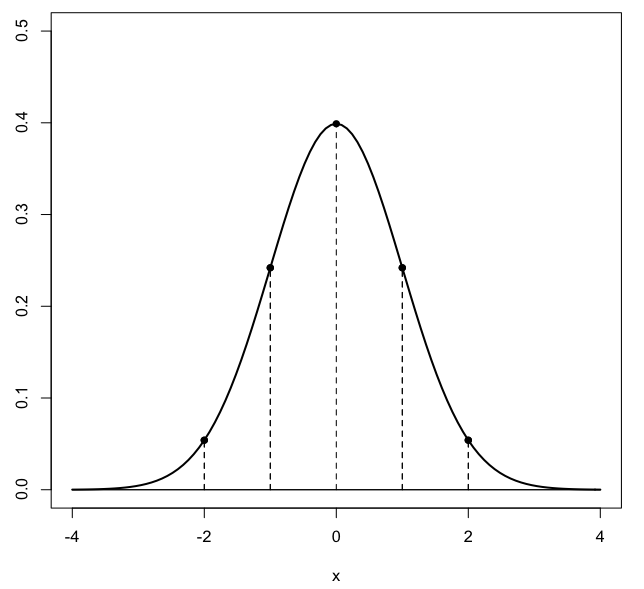
\includegraphics [scale=0.4] {gauss3.png} \end{center}

\title{Circular segment}
\date{}

\begin{document}
\maketitle
\Large

I found a hard geometry problem on the web:
\begin{center} 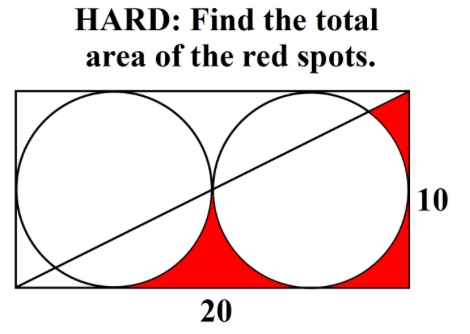
\includegraphics [scale=0.4] {circ_seg_prob.png} \end{center}
We know it's hard because it says so!

I liked it particularly because there are at least four different ways to calculate the answer using basic geometry and trigonometry, plus standard integration as well as polar integration.  I got the same answer each time, so I have increased confidence in the result.

It is included here because it's a fun problem, and one of the methods was polar integration to find the area.

As a first step, we observe that the problem has been made artificially complicated by using these particular values for the side lengths.  If both dimensions are scaled down by a factor of 5, then we obtain a rectangle with side lengths $4$ and $2$.  The two circles become unit circles.  We must just remember to re-scale to obtain the final answer, multiplying areas by $25$.

The area of any arched corner segment is pretty easy, since $4$ of them put together are equal to the difference between the area of a square with side length $2$ and a unit circle:  $4 - \pi$, so each one is $1 - \pi/4$.

The real difficulty is the upper right-hand corner.
\begin{center} 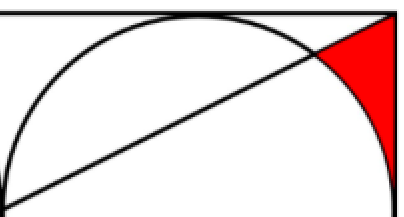
\includegraphics [scale=0.25] {circ_seg_prob2.png} \end{center}
One of the arches is divided into two pieces, and we are supposed to only count the red part of the arch.

The basic right triangle that we see repeated in these images has side lengths in the ratio $1:2$.  Its area is just $1$, and the smaller angle is 
\[ \phi = \tan^{-1} 0.5 \approx 0.4636 \text{ rad } \approx  26.565 \text{ deg } \]

\begin{center} 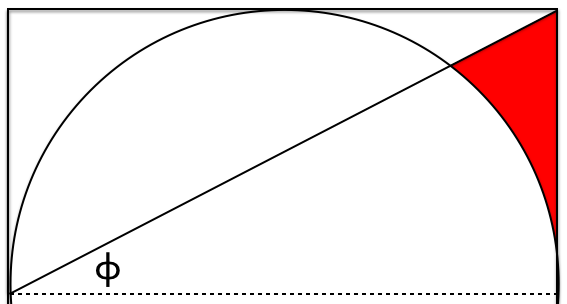
\includegraphics [scale=0.4] {circ_seg3.png} \end{center}
That's not a nice round number, but OK.
 
My first thought was to calculate the area cut off by the chord of a circle, called a "circular segment".  Then we could calculate the white part of the divided arch:
\[ \text{ triangle } - \text{ segment }  - \text{ arch } \]
\[ 1 - \text{ segment }  - (1 - \pi/4) \]

and subtract that from one whole arch to get the red part.
\[ (1 - \pi/4) - \ [ \ 1 - \text{ segment }  - (1 - \pi/4) \ ] \]
\[ 1 -  \frac{\pi}{2}  + \text{ segment } \]

We will use this result at the end for our final answer.  

There is an easier way, which we find by exploring this direction just a little further.

A circular segment is like a polar cap, but in two dimensions.
\begin{center} 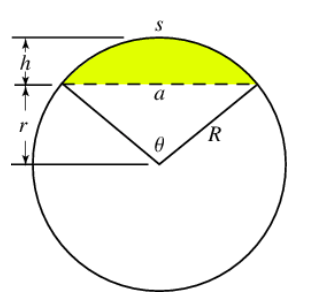
\includegraphics [scale=0.6] {circ_seg.png} \end{center}

\url{http://mathworld.wolfram.com/CircularSegment.html}

We carefully distinguish between the circular segment, in yellow, and the circular sector, which is the area of that slice of the circular pie swept out by the angle $\theta$.  

The area of the circular sector with central angle $\theta$ is the fraction of the total circular angle, times the area of a unit circle.  The result is just half the angle.
\[ \frac{\theta}{2 \pi} \cdot \pi = \frac{\theta}{2} \]

For the actual calculation of a circular segment, we would need not only the angle $\theta$, but also $r$ and $a$, which we would need to derive from $\theta$ by applying the Pythagorean theorem and/or trigonometry.  It can be done!  However, we see a better way.  

\subsection*{isosceles triangles}

The first key idea to draw $\theta$ on our diagram, and realize that $\theta$ is the apex angle of an isosceles triangle.  The two sides are both radii of our circle, and so are equal to each other!  Therefore $\theta = \pi - 2 \phi$.
\begin{center} 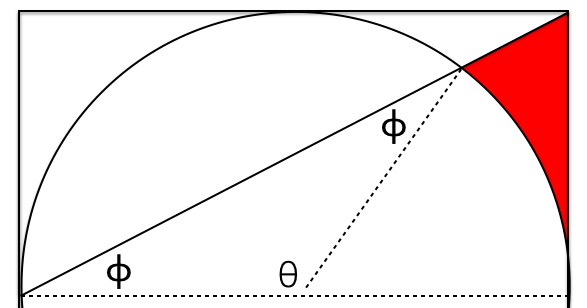
\includegraphics [scale=0.4] {circ_seg2.png} \end{center}

So now we just calculate the circular sector swept out by $\theta$ and figure out the area of the isosceles triangle, subtract to find the spherical segment and go on from there.  The beauty of this is we do not need to know the formulas for circular segments..

Let's continue by finding the lengths and areas of parts of the central isosceles triangle with angles $\phi$-$\phi$-$\theta$.

\begin{center} 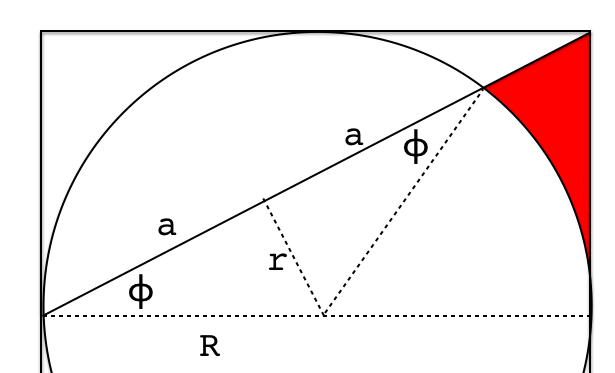
\includegraphics [scale=0.4] {circ_seg4.png} \end{center}
The triangle area is easy because one-half of it is a triangle similar to the original.  This means that $r/a = \tan \phi = 0.5$ so $a/r = 2$ and
\[ a = 2r \]
Furthermore
\[ r = R \sin \phi \]
\[ a = R \cos \phi \]

The area of the entire isosceles triangle is two of these smaller ones:
\[ A = ar = R^2 \sin \phi \cos \phi \]

We can also do it solely in terms of $r$
\[ A = 2r^2 \]
\[ = 2 R^2 \sin^2 \phi \]
For this unit circle
\[ A = 2 \sin^2 \phi \]

This works because 
\[ \cos \phi = 2 \sin \phi \] 
so
\[  \sin \phi \cos \phi = 2 \sin^2 \phi \]

Because of the square we get an exact answer:
\[ \sin \phi = \frac{1}{\sqrt{5}} \]
\[ \sin^2 \phi = \frac{1}{5} \]
\[ A = 2 \sin^2 \phi = 0.4 \]

Later, we will have a use for $h$:
\[ h = R - r = R(1 - \sin \phi) \]
\[ = 1 - \sin \phi \]

We could now move on to consideration of the circular sector with angle $\theta$.  But wait!

\subsection*{the other triangle}

Notice at this point a different circular sector, just to the right of the isosceles triangle.  Several different familiar theorems gives the angle as $2\phi$.

$\circ$\ \ \ $\theta + \phi + \phi = \pi$ but at the same time $\theta$ plus the unknown angle also equals $\pi$.  Thus, the angle is $2 \phi$.

$\circ$\ \ \ $\phi$ and the unknown angle both sweep out the same arc on the circle, but the unknown angle is at the origin of the circle, and $\phi$ is on the perimeter.  A famous theorem says the the unknown angle is twice $\phi$.  The same argument in reverse is a \emph{proof} of the theorem.

$\circ$\ \ \  Draw a horizontal line (not shown) intersecting the angled line and the perimeter of the circle, at the upper-right, just above and to the right of the letter $\phi$.  The angle between the new horizontal and the angled line is $\phi$, by another famous theorem (interior angles ...), and thus the unknown angle is twice $\phi$, by that same famous theorem.

\begin{center} 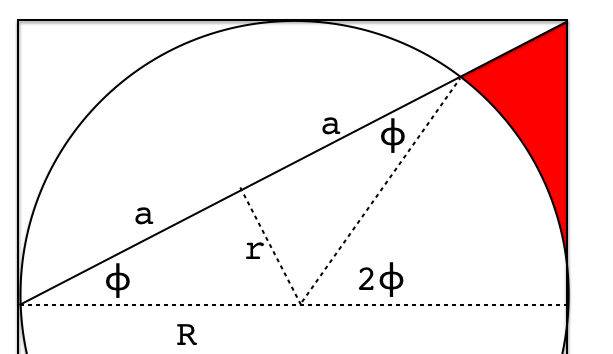
\includegraphics [scale=0.4] {circ_seg5.png} \end{center}

The area of the sector is, by the same calculation we did before, the ratio of the angle to $2 \pi$ times the area of the unit circle.
\[ \frac{2 \phi}{2 \pi} \ \pi = \phi \]

\subsection*{calculation 1:  ignore the circular segment}
So far we have that the area of the isosceles triangle is $2 \sin^2 \phi = \sin \phi \cos \phi$.

The circular sector with angle $2 \phi$ has area $\phi$.

The part of the large lower triangle that is not in red is
\[ \text{ circular sector } + \text{ isosceles triangle } \]
\[ \phi + 2 \sin^2 \phi \]

Then what we want is to subtract that from the large triangle:
\[ A = 1 - \phi - 2 \sin^2 \phi \]
\[ = 1 - \approx 0.46 - 0.4 \]
I get $\approx 0.14$, which seems reasonable.  

Let's try to remember that:  the red part of the arch is $1 - \phi - 2 \sin^2 \phi$.

\subsection*{calculation two:  polar area}
We can also use calculus, namely to compute a polar area.  Look again at
\begin{center} 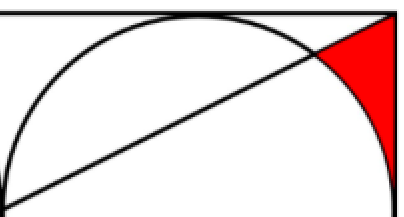
\includegraphics [scale=0.25] {circ_seg_prob2.png} \end{center}

What if we could get the area of the lower triangle minus the red part?

This is a pretty easy integral in polar coordinates.  Since the angle is usually given as $\theta$, for the moment we relabel $\phi$ as $\theta$.  We also reuse the variable $a$.

Set up a circle of radius $a$ with its left edge at the origin, the equation of that circle in polar coordinates is
\[ r = 2 a \cos \theta \]

For example, radius $a = 1$ gives
\[ \text{at } \theta = 0, \ \ \ \ r = 2 \]
\[ \text{at } \theta = \frac{\pi}{4}, \ \ \ \ r = \sqrt{2} \]
\[ \text{at } \theta = \frac{\pi}{2}, \ \ \ \ r = 0 \]
The arc of the upper semi-circle that we're seeing is $\theta = 0 \rightarrow \frac{\pi}{2}$

\[ \text{at } \theta = \phi, \ \ \ \ r = 2 \cos \phi  \]
Since $\cos \phi = 2 / \sqrt{5}$, $r = 4/\sqrt{5}$.

You don't believe me that this is correct?  We have four equations.  Always:
\[ r^2 = x^2 + y^2 \]
\[ x = r \cos \theta  \]
\[ y = r \sin \theta  \]
\emph{Do not cancel} the $r = 1$ yet.

We also have the equation of this circle.  The general equation is
\[ r = 2h \cos \theta + 2k \sin \theta \]
where $(h,k)$ is the origin of the circle.  Here, the origin is at $h = 1$ so
\[ r = 2 \cos \theta \]

Now comes the magic.  Substitute for $\cos \theta $:
\[ r = 2 \frac{x}{r} \]
\[ r^2 = 2 x \]
but
\[ r^2 = x^2 + y^2  \]
We obtain
\[ x^2 + y^2 = 2x \]
\[ x^2 - 2x + y^2 = 0 \]
Complete the square and add the same term on the right
\[ (x - 1)^2 + y^2 = 1 \]
This is indeed a unit circle with origin at $(1,0)$.

\subsection*{polar area}

The area is made up of many small wedges with angle $\theta$, and $r = f(\theta) = 2 \cos \theta $.  The wedges are approximately triangles with area $1/2 \cdot r \cdot r \ d \theta$.  So the total area is

\[ A = \int \frac{1}{2} \ [ \ f(\theta) \ ]^2 \ d \theta \]

\[ = \frac{1}{2} \ 4 \int \cos^2 \theta \ d \theta\]
\[ = 2 \ [ \ \frac{1}{2} (\theta + \sin \theta \cos \theta) \ ] \ \bigg |_0^{\phi} \]
At the lower bound, this is zero so
\[ A = \phi + \sin \phi \cos \phi \]

For this $\phi$ we have that:
\[ A = \phi + 2 \sin^2 \phi \]

This should be equal to the area of the circular sector of angle $2 \phi$ plus the area of the isosceles triangle, and if you look back, you'll see that we have a match.

To get the red arch, we must subtract this from the triangle, which has unit area.
\[ A = 1 - \phi - 2 \sin^2 \phi \]

That matches what we had before.  To finish up, we do this two more ways, both requiring the area of the circular segment.

\subsection*{calculation 3:  standard calculus}
We find the circular segment by standard integral calculus:

\begin{center} 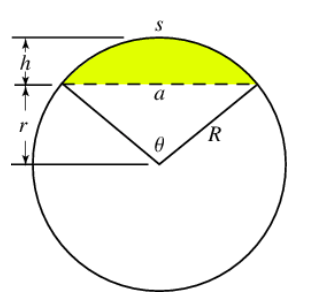
\includegraphics [scale=0.6] {circ_seg.png} \end{center}
Recall that the area of (the upper half of) a circle drawn in standard orientation ($x$ horizontal) is
\[ \int \sqrt{R^2 - x^2} \ dx \]
The bounds we need are $R-h$ to $R$.  

Here we have rotated a quarter-turn and are integrating vertically, so we'll use $y$ as the variable.  The area of the half-circle to the right of the $y$-axis is
\[ \int_{R-h}^R \sqrt{R^2 - y^2} \ dy \]

This is a unit circle so
\[ A = \int_{1-h}^1 \sqrt{1 - y^2} \ dy \]
The answer (done many times by now)
\[ \frac{1}{2} \ [ \ \sin^{-1} y + y \sqrt{1 - y^2} \ ]  \ \bigg |_{1-h}^1 \]

At the upper bound we get $\pi/4$.  For the lower bound we need $h$
\[ h = 1 - \sin \phi \]
so that bound is just $\sin \phi$.
The first term in parentheses is
\[ \sin^{-1} (\sin \phi) \]
The angle whose sine is $\sin \phi$ is just $\phi$!

The second term is
\[ (\sin \phi) \sqrt{1 - (\sin \phi)^2} \]
\[ = \sin \phi \cos \phi \]
Altogether, we have 
\[ \frac{\pi}{4} - \frac{1}{2} (\phi + \sin \phi \cos \phi) \]
\[ = \frac{\pi}{4} - \frac{\phi}{2} - \sin^2 \phi  \]
This is (almost) the circular segment.

It is off by a factor of 2.  The reason is that the integral only gives the area of that part of the circle that is above the $x$-axis.  We must multiply the provisional answer by $2$.
\[ = \frac{\pi}{2} - \phi - 2 \sin^2 \phi  \]

Wait for the calculation of the red part of the arch, starting from the circular segment.

\subsection*{calculation four:  geometry}

\begin{center} 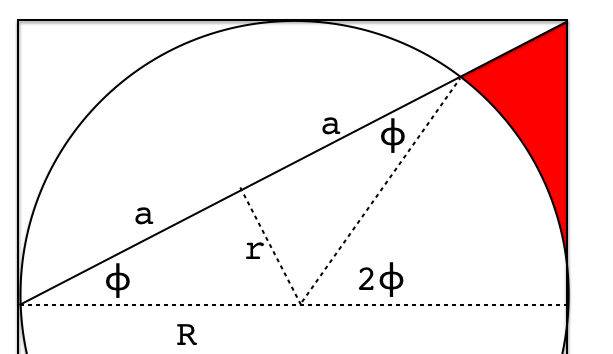
\includegraphics [scale=0.4] {circ_seg5.png} \end{center}
We have that the area of the isosceles triangle is exactly 
\[ \sin \phi \cos \phi = 2 \sin^2 \phi = 0.4 \]

The area of the circular sector with angle $\theta$ is 
\[ \frac{\theta}{2 \pi} \ \pi =  \frac{\theta}{2} \]

in terms of angle $\phi$:
\[ = \frac{1}{2} (\pi - 2 \phi) \]
\[ = \frac{\pi}{2} - \phi \]

The area of the circular segment is the area of the circular sector minus that of the isosceles triangle:
\[ \frac{\pi}{2} - \phi - 2 \sin^2 \phi \]
This matches what we had for the third calculation, by integration of the equation of the circle.

\subsection*{the red part of the arch}
At the very beginning we calculated the red part of the arch as:
\[ 1 -  \frac{\pi}{2}  + \text{ segment } \]

Now we have the circular segment with angle $\theta$ (in terms of $\phi$) as 
\[ \frac{\pi}{2} - \phi - 2 \sin^2 \phi \]

So the answer for the red part of the arch is
\[ 1 -  \frac{\pi}{2}  + \frac{\pi}{2} - \phi - 2 \sin^2 \phi \]
\[ 1 - \phi - 2 \sin^2 \phi \]

This matches parts one and two.  All four methods give the same answer, which is quite a relief.

\subsection*{finishing up}
To meet the problem statement, we must add this fractional arch to $3$ complete copies, and then multiply the whole thing by the square of the scaling factor (because this is an area):

\[ 25 \ [ 1 - \phi - 2 \sin^2 \phi \ + 3(1 - \pi/4) \ ] \]
I'm too tired to calculate it.

\begin{center} 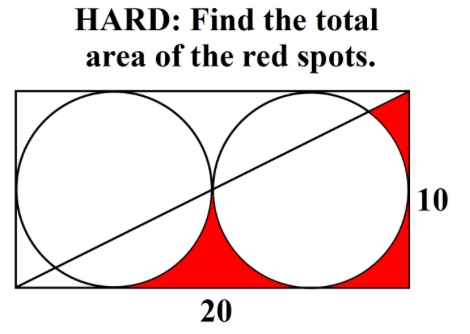
\includegraphics [scale=0.4] {circ_seg_prob.png} \end{center}

\subsection*{A fifth way}

Later on, I thought of another approach, also pretty simple.  Recall the point described in words way back in the section on \textbf{the other triangle}.  

Here, that point is shown in cyan:

\begin{center} 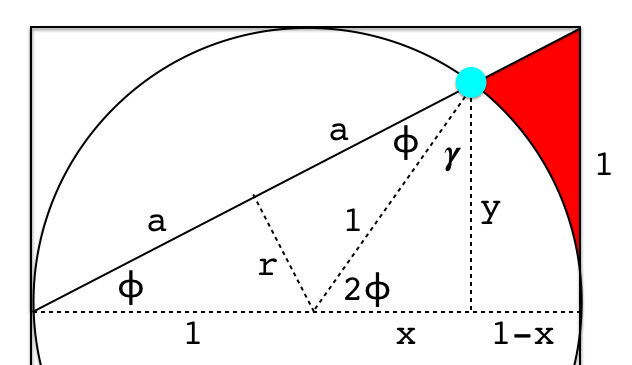
\includegraphics [scale=0.4] {circ_seg6.png} \end{center}

From the diagram we can see that
\[ \frac{y}{2a} = \sin \phi \]
\[ y = 2 a \sin \phi  \]

To get $x$ and $y$ in terms of only $\phi$ we can proceed as follows.  A basic result we obtained before was that
\[ a = \cos \phi = 2 \sin \phi \]
so
\[ y = 2a \sin \phi \]
\[ = 4 \sin^2 \phi \]
\[ = \cos^2 \phi \]
\[ = (\frac{2}{\sqrt{5}})^2 = \frac{4}{5} \]

$x$ looks more complicated but since $x^2 + y^2 = 1$, we can at least calculate $x = 3/5$.

Notice that 
\[ y = \sin 2 \phi \]
and by the double-angle formula
\[ y = 2 \sin \phi \cos \phi = \cos^2 \phi \]
as before.  

So for $x$ we have
\[ x = \cos 2 \phi \]
\[ = \cos^2 \phi - \sin^2 \phi \]
\[ = 2 \cos^2 \phi - 1 = 2 y - 1 \]

which is confirmed by doing the arithmetic.

Redraw the figure slightly

\begin{center} 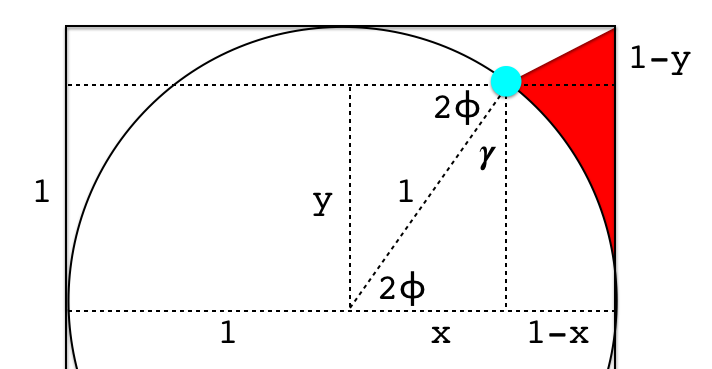
\includegraphics [scale=0.4] {circ_seg7.png} \end{center}

Notice that part of the red arch is the area to the right of the circle, and the rest is a triangle.

Let $x = f(y) = \sqrt{1-y^2}$ be the function and calculate the relevant area (the part of the circle in the first quadrant lying below the horizontal line at $y$) as

\[ A = \int_0^y \sqrt{1-y^2} \ dy \]
\[ = \frac{1}{2} \ [ \sin^{-1} y + y \ \sqrt{1-y^2} \ ] \ \bigg |_0^y \]

At the lower bound everything is zero and at the upper bound
\[ A = \frac{1}{2} (\sin^{-1} y + y \ \sqrt{1-y^2}) \]

From the figure, we can see that $2 \phi = \sin^{-1} y$ so
\[ A = \frac{1}{2} (2 \phi + xy) \]
\[ = \phi + \frac{xy}{2} \]
Leave this as it is for the moment.

The area of the red arch below the horizontal line is $y$ minus this.
\[ A = y - \phi - \frac{xy}{2} \]

Finally we must add the area of the triangle above.  That area is
\[ \frac{1}{2} (1-x)(1-y) \]
\[ = \frac{1}{2}  (1 - x - y + xy)  \]

Putting it all together
\[ A = y - \phi - \frac{xy}{2} +  \frac{1}{2}  (1 - x - y + xy)  \]
The $xy$ terms cancel.
\[ A = y - \phi +  \frac{1}{2}  (1 - x - y)  \]
Recall that $x = 2y - 1$
\[ A = y - \phi +  \frac{1}{2}  (1 - 2y + 1  - y)  \]
\[ = 1 - \phi - \frac{1}{2} y \]
And $y = 4 \sin^2 \phi$ so
\[ A = 1 - \phi - 2 \sin^2 \phi \]

This matches what we had before.  

We obtained the same area five ways (well, at least four ways, two are variants of each other).

\end{document}